\documentclass{article}

\usepackage{graphicx}
\usepackage{tikz}
\usepackage{tikzsymbols}
\usetikzlibrary{calc,patterns,shapes.geometric}
\pagestyle{empty}
\usepackage[margin=0pt]{geometry}
\geometry{papersize={14in,12in}}

\def\centerarc[#1](#2)(#3:#4:#5){\draw[#1] ($(#2)+({#5*cos(#3)},{#5*sin(#3)})$) arc (#3:#4:#5);}

\begin{document}
	\begin{figure}
		\centering
		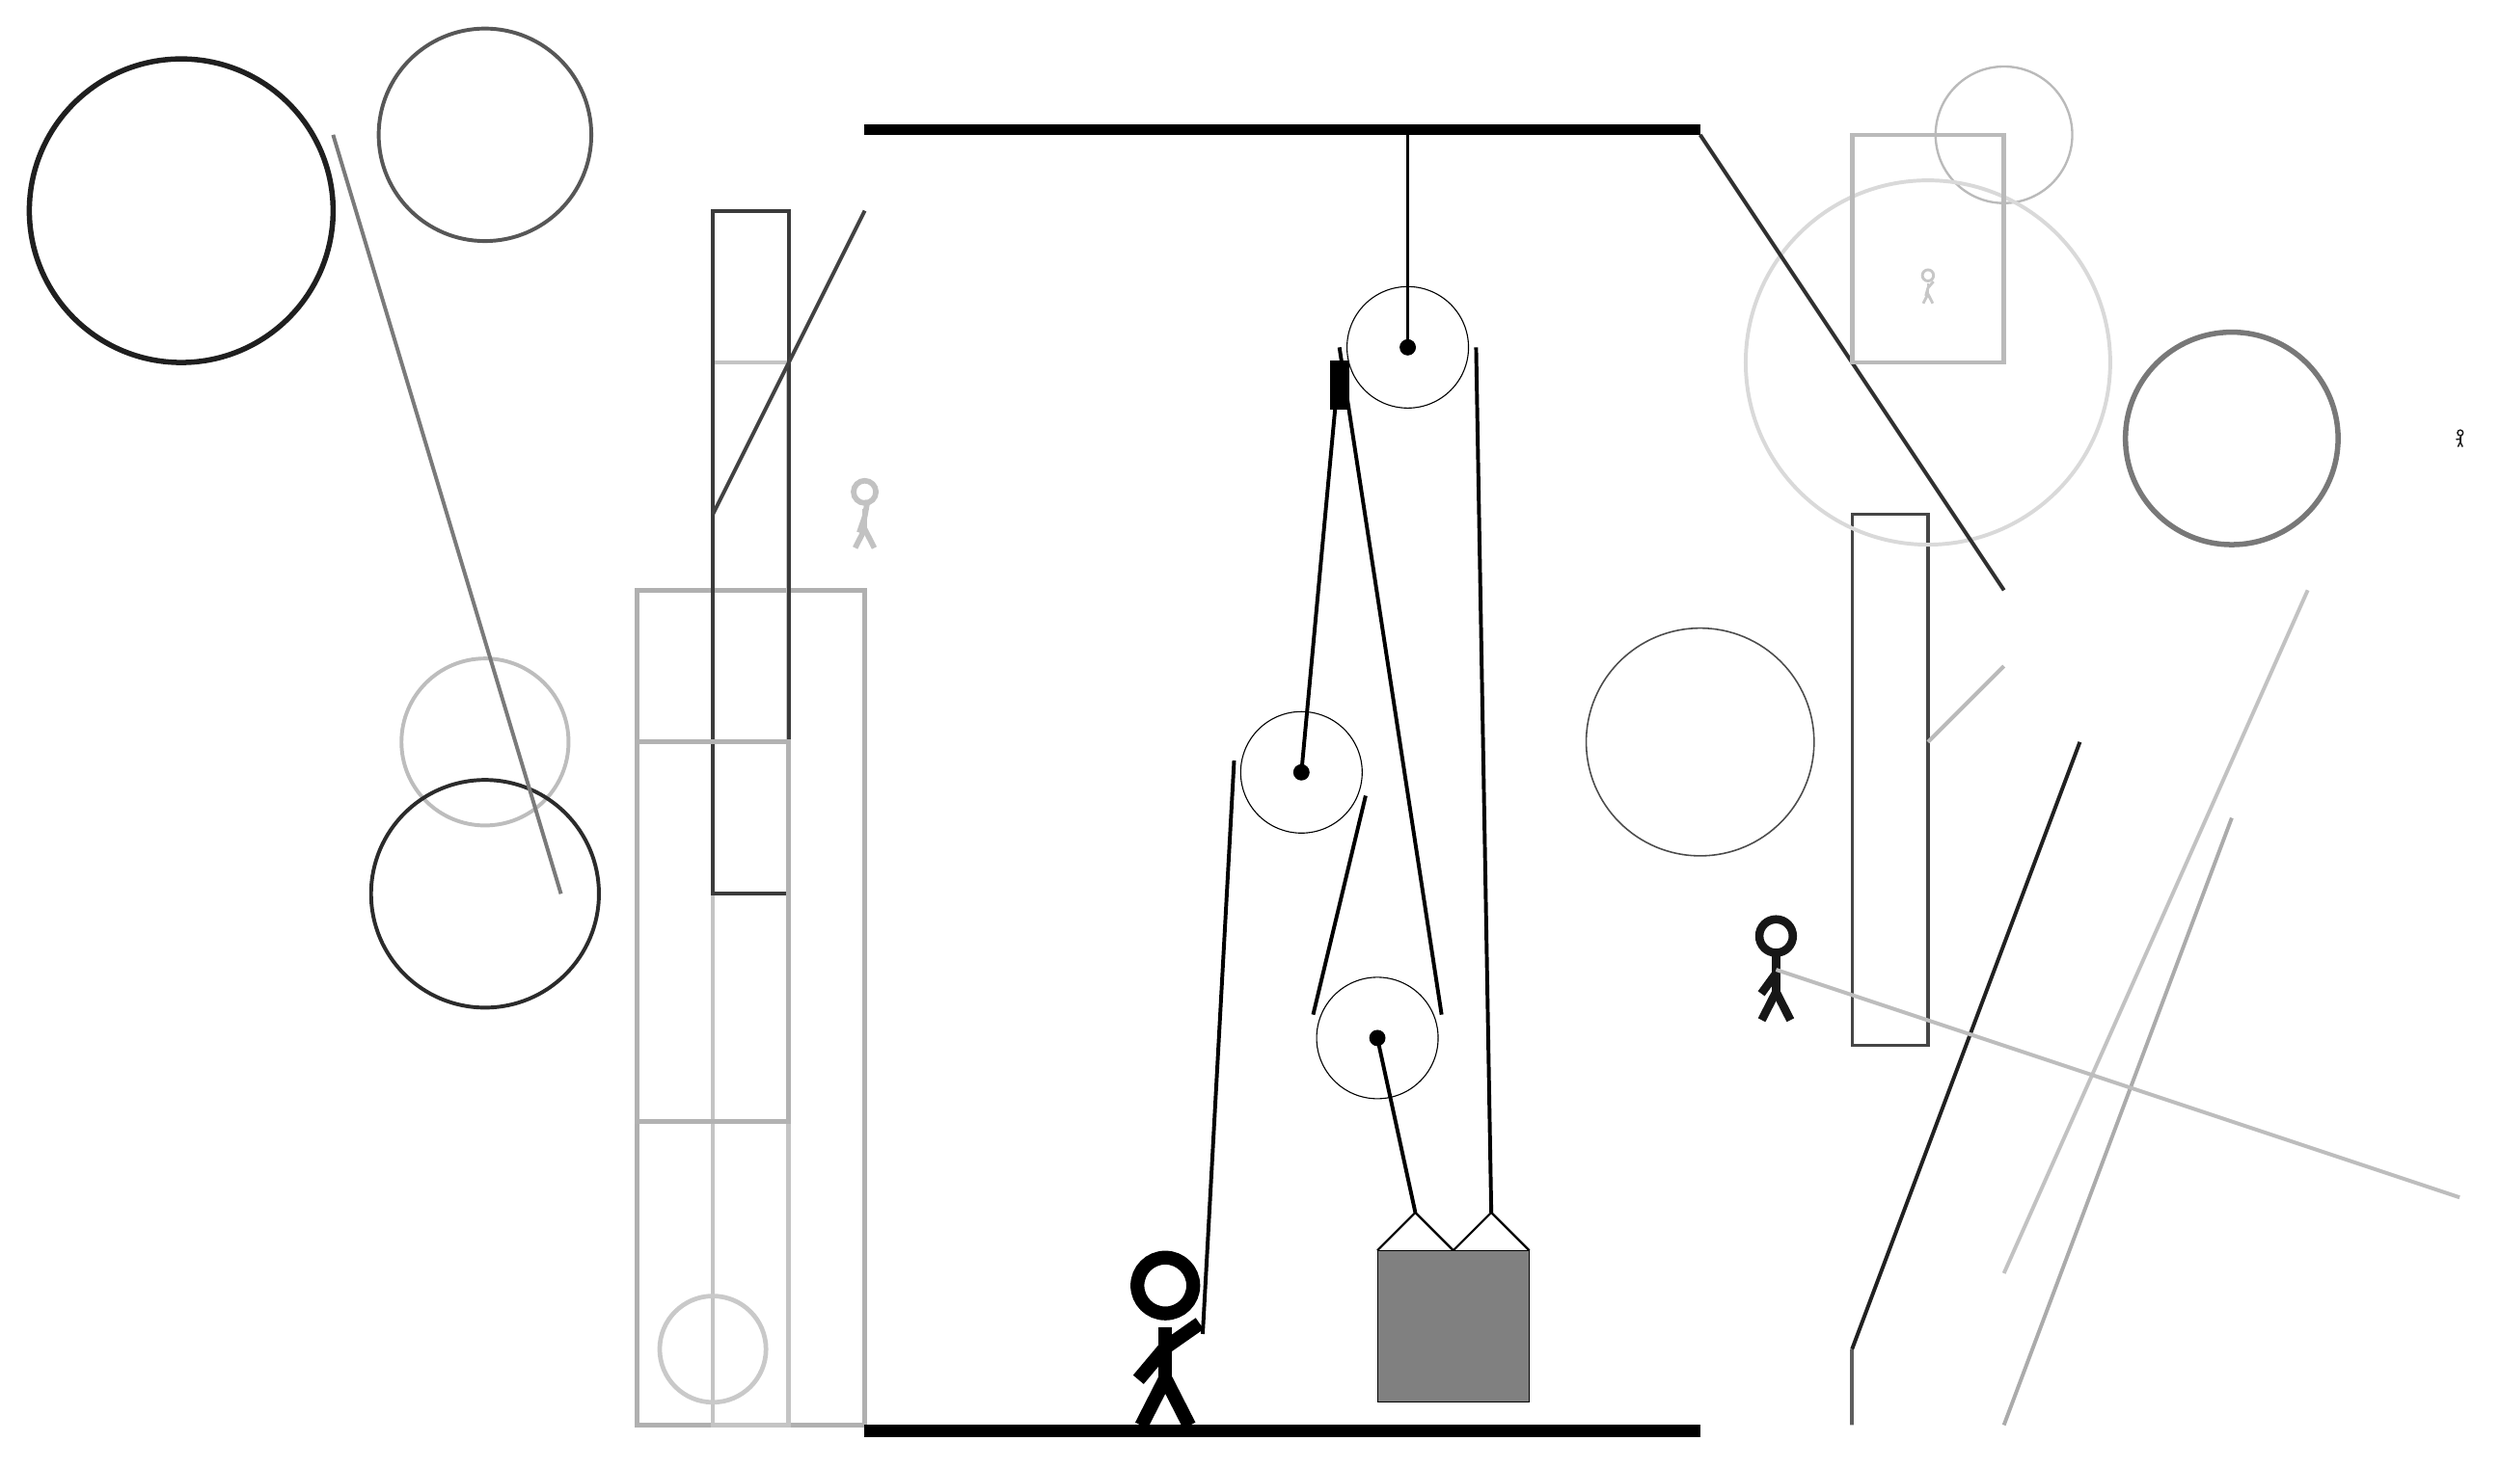
\begin{tikzpicture}
			%%%%% START %%%%%
			
			\draw[fill=black] (-6, 14) rectangle (5, 14.125);
			
			\draw (-0.25, 5.6) circle (0.8);
			\draw[fill=black] (-0.25, 5.6) circle (0.1);
			
			\draw (0.75, 2.1) circle (0.8);
			\draw[fill=black] (0.75, 2.1) circle (0.1);
			
			\draw [line width=0.5mm, color=black!26](-11, 6) circle (1.1);
			
			\draw[line width=0.7mm, color=black!31] (-6, -3) rectangle (-9, 8);
			\draw[line width=0.6mm, color=black!23] (-7, 11) rectangle (-8, -3);
			\draw[line width=0.5mm, color=black!24](9, -1) -- (13, 8);
			
			\node[line width=0.6mm, color=black!89] at (15, 10) {\Strichmaxerl[1][6][75]};
			\node[line width=0.4mm, color=black!22] at (8, 12) {\Strichmaxerl[2][75][49]};
			\draw[line width=0.5mm, color=black!77] (-7, 13) rectangle (-8, 4);
			\draw[line width=0.5mm, color=black!33](9, -3) -- (12, 5);
			\draw[line width=0.5mm, color=black!63] (7, -3) rectangle (7, -2);
			
			\draw[line width=0.6mm, color=black!30] (-7, 1) rectangle (-9, 6);
			
			\draw[line width=0.5mm, color=black!87](10, 6) -- (7, -2);
			\node[line width=0.4mm, color=black!91] at (6, 3) {\Strichmaxerl[6][54][90]};
			\draw[line width=0.4mm, color=black!73] (7, 9) rectangle (8, 2);
			
			\draw [line width=0.6mm, color=black!21](-8, -2) circle (0.7);
			\draw [line width=0.7mm, color=black!88](-15, 13) circle (2.0);
			\draw [line width=0.2mm, color=black!21](10, -1) circle (0.0);
			\draw [line width=0.3mm, color=black!27](9, 14) circle (0.9);
			\draw[line width=0.5mm, color=black!26](6, 3) -- (15, 0);
			\node[line width=0.2mm, color=black!24] at (-6, 9) {\Strichmaxerl[4][71][80]};
			\draw [line width=0.7mm, color=black!53](12, 10) circle (1.4);
			\draw [line width=0.5mm, color=black!15](8, 11) circle (2.4);
			
			\draw[line width=0.5mm, color=black!27](9, 7) -- (8, 6);
			\draw [line width=0.5mm, color=black!66](-11, 14) circle (1.4);
			\draw [line width=0.2mm, color=black!70](5, 6) circle (1.5);
			\draw [line width=0.5mm, color=black!83](-11, 4) circle (1.5);
			
			\draw[line width=0.5mm, color=black!74](-8, 9) -- (-6, 13);
			
			\draw[line width=0.5mm, color=black!81](5, 14) -- (9, 8);
			\draw[line width=0.6mm, color=black!27] (7, 11) rectangle (9, 14);
			\draw[line width=0.5mm, color=black!52](-10, 4) -- (-13, 14);
			
			
			\draw (1.15, 11.2) circle (0.8);
			\draw[fill=black] (1.15, 11.2) circle (0.1);
			\draw[very thick] (1.15, 11.2) -- (1.15, 14);
			
			\draw[thick]  (0.75, -0.7) -- (1.25, -0.2) -- (1.75, -0.7) -- (2.25, -0.2) -- (2.75, -0.7);
			\draw[fill=black!50] (0.75, -0.7) rectangle (2.75, -2.7);
			
			\draw[line width=0.5mm] (-0.25, 5.6) -- (0.25, 11.0);
			\draw[line width=0.5mm, fill=black](0.15, 10.4) rectangle (0.35, 11.0);
			\draw[line width=0.5mm] (-1.55, -1.8) -- (-1.1363, 5.7562);
			\centerarc[line width=0.5mm](-0.25, 5.6)(-20:170:0.9);
			\draw[line width=0.5mm] (0.5957, 5.2922) -- (-0.0957, 2.4078);
			\centerarc[line width=0.5mm](0.75, 2.1)(160:380:0.9);
			\draw[line width=0.5mm] (1.5957, 2.4078) -- (0.25, 11.2);
			\draw[line width=0.5mm](0.75, 2.1) -- (1.25, -0.2);
			\centerarc[line width=0.5mm](1.15, 11.2)(0:180:0.9);
			\draw[line width=0.5mm] (2.05, 11.2) -- (2.25, -0.2);
			
			\node at (-2, -1.9) {\Strichmaxerl[10][50][35]};
			
			\draw[fill=black] (-6, -3) rectangle (5, -3.15);
			
			%%%%% END %%%%%
		\end{tikzpicture}
	\end{figure}	
\end{document}